\documentclass[../main.tex]{subfile}
\begin{document}
\section{Physical principle}
\subsection{The force field}
    The laws of electrostatics or more presicly the Coulomb force is described as a force that attracts or repulses a 
    particle based on its distance from a well/source. This is quite simple, if your are nearer to one of this so called
    extremas, you're going to expreience a stronger force than from an other extrema.\\

    Now where does the force of an extrema point at? If we draw a line from the extremum to a particle,
    the force will act on this line and point towards the extremum if we are in an attractive setup and outward if we are in
    the repsulive case.\\

    The total picture is then represented as a sum over all forces as Newton describes it. Put in a mathematical way we have for the force of one extremm $i$:

    \begin{equation}
        F_{\text{extr},i}(\bm{r}) = I_i\cdot\frac{\bm{r}-\bm{r}_i}{||\bm{r}-\bm{r}_i||_2^2} 
    \end{equation}
    With $\bm{r}_i$ the location of the source and $I_i$ its influence power. This value is negative for a well such that the force
    points towards the well.
    For the booster we add the force in the direction that the booster points at and modualte with the distance.
    \begin{equation}
        F_{\text{boost},i}(\bm{r}) = I_i\cdot\frac{\bm{k}_i}{||\bm{r}-\bm{r}_i||_2^p} 
    \end{equation}
    where $\bm{k}_i$ describes the pointing vector of the boost. Tweeking the power $p$ we can make the force more sharp or more fallten. This is the \texttt{power} 
    parameter in the Blueprints.\\
     We now have $n\in[0,N_e]$ with $N_e$ the number of extrema and
    $m\in[0,N_b]$, $N_b$ the number of boosts. We then can write for the total force experienced at a location $\bm{r}$:

    \begin{equation}
        F_{\text{wind}}(\bm{r}) = \sum_n F_{\text{extr},n}(\bm{r}) + \sum_m F_{\text{boost},i}(\bm{r})
    \end{equation}
    This function is stored in the \texttt{BP\_WindManager::GetWindAtLocation methode}. For those unknown with this notation it means
    \texttt{ObjectWhereTheFunctionIsStored::TheFunction}. In cpp the object is a class, but UE5 on the editor side has a class per file.
    \begin{figure}[H]
        \centering
        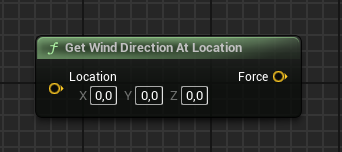
\includegraphics[width=0.3\textwidth]{Ressources/GetWindAtLoc.png}
    \end{figure}
\subsection{Derivation of a position update}
    We can simply use the newton lays of motion to derive the position update. We have for a mass of $m=1$
    \[
        \bm{F}(t) = m\cdot\bm{a}(t) \Leftrightarrow \bm{a}(t) = \frac{\bm{F}(t)}{m}.
    \]
    Knowing $\frac{\text{d}\bm{v}(t)}{\text{d}t} = \bm{a}(t)$, we can get the velocity by integrating the acceleration over the time:

    \[
        \bm{v}(t) = \int \bm{a}(t)\text{d}t = t\cdot\bm{a}(t) + \bm{v}_0
    \]
    and knowing that $\frac{\text{d}\bm{r}(t)}{\text{d}t} = \bm{v}(t)$ or the usaly ``velocity equals distance over time'' we obtain:
    \begin{equation}\label{eq:position}
        \bm{r}(t) = \int \bm{v}(t)\text{d}t = \frac{1}{2}t^2\cdot\bm{a}(t) + \bm{v}_0\cdot t + \bm{r}_0
    \end{equation}
    $\bm{r}_0$ is the initial position of the particle and $\bm{v}_0$ the initial velocity. This are constant that adds up when we integrate.\\
\end{document}